\documentclass[a4paper,11pt]{article}
\usepackage[a4paper, margin=2.5cm]{geometry}
\usepackage[utf8]{inputenc}
\usepackage{graphicx}
\usepackage{caption}
\usepackage{subcaption}
\usepackage{float}
\usepackage{amsmath}
\usepackage{pgfplots}
\usepackage{ffcode}
\usepackage{booktabs}
\usepackage{xcolor}
\usepackage{listings}
\usepackage{array}
\usepackage{tikz}
\usepackage{algorithm}
\usepackage{algpseudocode}
\usetikzlibrary{calc,patterns,angles,quotes}

\pgfplotsset{compat=1.18} 

\makeatletter
\newenvironment{breakablealgorithm}
{% \begin{breakablealgorithm}
\begin{center} %
\refstepcounter{algorithm}% New algorithm
%\hrule height.8pt depth0pt \kern2pt% \@fs@pre for \@fs@ruled
\hrule height.8pt depth0pt \kern2pt% \@fs@pre for \@fs@ruled
\renewcommand{\caption}[2][\relax]{% Make a new \caption
{\raggedright\textbf{\ALG@name~\thealgorithm} ##2\par}
\ifx\relax##1\relax
\addcontentsline{loa}{algorithm}{\protect\numberline{\thealgorithm}##2}%
\else
\addcontentsline{loa}{algorithm}{\protect\numberline{\thealgorithm}##1}%
\fi
\kern2pt\hrule\kern2pt
}
}{% \end{breakablealgorithm}
\kern2pt\hrule\relax% \@fs@post for \@fs@ruled
\end{center} %
}
\makeatother

\begin{document}
	
\title{
	\textbf{Quadson}
}
\author{Ying Pei Lin}
\date{Spring 2025}
\maketitle

\section{Introduction}

Quadson is a 3D printed quadruped robot designed as a platform for exploring advanced robotic motion and control.
This document includes its forward kinematics, inverse kinematics, differential kinematics and expands to body kinematics and locomotion.
Following the analysis, we will introduce the process of performing simultion in Pybullet and using deep
reinforcement learning to improve the robot's control and performance.

\section{Forward Kinematics}

For each leg of the robot, we define the reference frame with its origin at point $p_1$. 
Two motors are positioned at $p_1$ and $p_5$ respectively, and the third motor
connected to the entire leg assembly, controls the rotation around x axis. The remaining joints in the leg are all passive.

\begin{center}
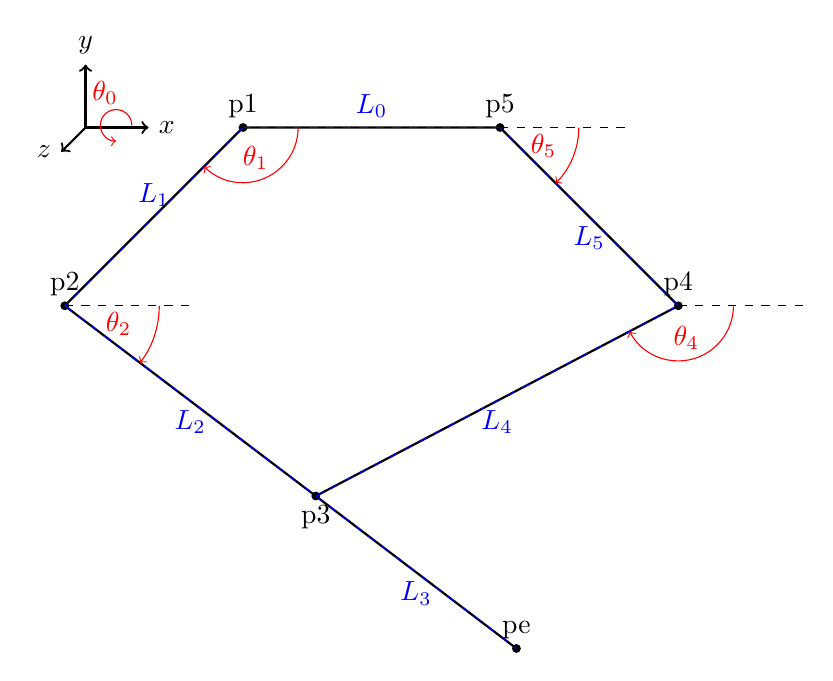
\begin{tikzpicture}[scale=0.4]
	% Points
	\coordinate (p1) at (0,0);
	\coordinate (p2) at (-5.66,-5.66);
	\coordinate (p2_hori) at (-1.66,-5.66);
	\coordinate (p3) at (2.31,-11.70);
	\coordinate (pe) at (8.68,-16.54);
	\coordinate (p4) at (13.82,-5.66);
	\coordinate (p4_hori) at (17.82,-5.66);
	\coordinate (p5) at (8.16,0);
	\coordinate (p5_hori) at (12.16,0);

	% Lines
	\draw[thick] (p1) -- (p2) -- (p3) -- (p4) -- (p5) -- (p1);
	\draw[thick] (p3) -- (pe);
	\draw[dashed] (p2) -- (p2_hori);
	\draw[dashed] (p4) -- (p4_hori);
	\draw[dashed] (p5) -- (p5_hori);
	
	% Axis
	\draw[thick,->] (-5,0,0) -- (-3,0,0) node[right] {$x$};
	\draw[thick,->] (-5,0,0) -- (-5,2,0) node[above] {$y$};
	\draw[thick,->] (-5,0,0) -- (-5,0,2) node[left] {$z$};
	\draw[red,->] (-3.8,-0.2,-0.7) arc[start angle=0,end angle=270,radius=0.5cm] node[midway,above] {$\theta_0$};

	% Point tags
	\foreach \p in {p1, p2, pe, p4, p5} {
			\fill[black] (\p) circle (4pt);
			\node[above] at (\p) {\p};
	}
	\fill[black] (p3) circle (4pt);
	\node[below] at (p3) {p3};

	% Length tags
	\draw[blue, dashed] (p1) -- (p5) node[midway, above] {$L_{0}$};
	\draw[blue, dashed] (p1) -- (p2) node[midway, above] {$L_{1}$};
	\draw[blue, dashed] (p2) -- (p3) node[midway, below] {$L_{2}$};
	\draw[blue, dashed] (p3) -- (pe) node[midway, below] {$L_{3}$};
	\draw[blue, dashed] (p3) -- (p4) node[midway, below] {$L_{4}$};
	\draw[blue, dashed] (p4) -- (p5) node[midway, below] {$L_{5}$};

	% Angle tags
	\pic [draw=red, text=red, <-, "$\theta_1$", angle radius=0.7cm] {angle=p2--p1--p5};
	\pic [draw=red, text=red, <-, "$\theta_2$", angle radius=1.2cm] {angle=p3--p2--p2_hori};
	\pic [draw=red, text=red, <-, "$\theta_4$", angle radius=0.7cm] {angle=p3--p4--p4_hori};
	\pic [draw=red, text=red, <-, "$\theta_5$", angle radius=1cm] {angle=p4--p5--p5_hori};
\end{tikzpicture}
\end{center}

The following algorithm takes the angle of three motors as input and computes the position of the end-effector.

\begin{breakablealgorithm}
	\caption{Compute Leg End-Point}
	\begin{algorithmic}[1]
			\Require Motor angles $\theta_0, \theta_1, \theta_5$
			\State Compute initial 2D joint positions:
			\begin{align*}
				&p_2 = (L_1 \cos \theta_1, -L_1 \sin \theta_1), p_5 = (L_0, 0), \\
				&p_4 = p_5 + (L_5 \cos \theta_5, -L_5 \sin \theta_5)
			\end{align*}
			\State Compute distances:
			$$
					L_{14} = \| p_4 - p_1 \|, \quad
					L_{24} = \| p_4 - p_2 \|
			$$
			\State Solve for $p_3$ using angles:
			$$
					\theta_2 = \cos^{-1} \left( \frac{L_2^2 + L_{24}^2 - L_4^2}{2 L_2 L_{24}} \right) +
										 \cos^{-1} \left( \frac{L_1^2 + L_{24}^2 - L_{14}^2}{2 L_1 L_{24}} \right) - (\pi - \theta_1)
			$$
			$$
					p_3 = p_2 + L_2 (\cos \theta_2, -\sin \theta_2)
			$$
			\State Compute endpoint:
			$$
					p_e = p_2 + (L_2 + L_3)(\cos \theta_2, -\sin \theta_2)
			$$
			\State Transform to 3D using rotation matrix:
			$$
				R_{\theta_0} =
				\begin{bmatrix}
						1 & 0 & 0 \\
						0 & \cos(-\theta_0) & -\sin(-\theta_0) \\
						0 & \sin(-\theta_0) & \cos(-\theta_0)
				\end{bmatrix}, 
				p_e = R_{\theta_0} \times \begin{bmatrix} p_e[0] \\ p_e[1] \\ 0 \end{bmatrix}
			$$
			\State \Return $p_e$
	\end{algorithmic}
\end{breakablealgorithm}

\section{Inverse Kinematics}

In real world scenarios, controlling position of the end-effector to reach to a certain position
is often more pratical than setting the angles directly. For example, to move the end-effector along 
a defined trajectory, achieving this by manually adjusting the three motor angles is nearly impossible 
due to the complexity of the joint movements. 

Therefore we need the following algorithm 
to compute the angles of the motor corresponding to a given target position.

\begin{breakablealgorithm}
	\caption{Compute Joint Angles from End-Point}
	\begin{algorithmic}[1]
			\Require End-point position $(x, y, z)$
			\State Calculate angle of motor 0:
			$$
				\theta_0 = -\tan^{-1} \left( \frac{z}{-y} \right)
			$$
			\State Translate points from 3D to 2D using rotation matrix:
			$$
				R_{\theta_0} =
					\begin{bmatrix}
						1 & 0 & 0 \\
						0 & \cos(-\theta_0) & -\sin(-\theta_0) \\
						0 & \sin(-\theta_0) & \cos(-\theta_0)
					\end{bmatrix}
			$$
			$$
				\begin{bmatrix} x' \\ y' \\ z' \end{bmatrix} = R_{\theta_0} \times \begin{bmatrix} x \\ y \\ z \end{bmatrix}
			$$
			\State Calculate angle 1:
			$$
				L_{1e} = \| (x', y') \|, \quad
				\theta_{e15} = \tan^{-1} \left( \frac{-y'}{x'} \right)
			$$
			$$
				\theta_{e12} = \cos^{-1} \left( \frac{L_1^2 + L_{1e}^2 - (L_2 + L_3)^2}{2 L_1 L_{1e}} \right)
			$$
			$$
				\theta_1 = \theta_{e15} + \theta_{e12}
			$$
			\State Compute positions of joints:
			$$
				p_1 = (0, 0), \quad
				p_2 = (L_1 \cos \theta_1, -L_1 \sin \theta_1)
			$$
			$$
				p_3 = \frac{(pe_2d \cdot L_2) + (p_2 \cdot L_3)}{L_2 + L_3}, \quad
				p_5 = (L_0, 0)
			$$
			\State Calculate angle 5:
			$$
				\theta_{350} = \tan^{-1} \left( \frac{-p_3[1]}{L_0 - p_3[0]} \right)
			$$
			$$
				\theta_{354} = \cos^{-1} \left( \frac{L_{35}^2 + L_5^2 - L_4^2}{2 L_{35} L_5} \right), \quad
				L_{35} = \| p_3 - p_5 \|
			$$
			$$
				\theta_5 = \pi - (\theta_{350} + \theta_{354})
			$$
			\State \Return $(\theta_0, \theta_1, \theta_5)$
	\end{algorithmic}
\end{breakablealgorithm}

\section{Differential Kinematics}

To control a quadruped robot's leg smoothly, we employ differential kinematics, which provides the relation between joint angular velocities and linear velocity of the end-effector.

Given the motor angles $\boldsymbol{\theta} = [\theta_0, \theta_1, \theta_5]^T$ and their angular velocities $\dot{\boldsymbol{\theta}} = [\omega_0, \omega_1, \omega_5]^T$. 
The linear velocity of the end-effector $\mathbf{v} = [v_x, v_y, v_z]^T$ can be represented as following:

$$
\mathbf{v} = \mathbf{J}(\boldsymbol{\theta}) \cdot \dot{\boldsymbol{\theta}}
$$

Where $\mathbf{J}(\boldsymbol{\theta}) \in \mathbf{R}^{3 \times 3}$ is the Jacobian matrix. It is updated continuously as $\boldsymbol{\theta}$ 
changes during motion even if the given linear velocity remain the same.
Note that angular velocity of the end-effector ($\omega_x, \omega_y, \omega_z$) is ignored because the foot contact does not require rotational control in this context.

To find the inverse, the required motor angular velocities for a desired end-effector linear velocity can be represented as following:

$$
\dot{\boldsymbol{\theta}} = \mathbf{J}^{+}(\boldsymbol{\theta}) \cdot \mathbf{v}
$$

Where $\mathbf{J}^+$ is the Moore-Penrose pseudoinverse of $\mathbf{J}$.

\begin{algorithm}[H]
	\caption{Compute Joint Velocities from End-Effector Velocity}
	\begin{algorithmic}[1]
		\Require End-effector velocity $\mathbf{v} = [v_x, v_y, v_z]^T$
		\State Read current joint angles $\boldsymbol{\theta}$
		\State Compute forward kinematics to get $\mathbf{p} = f(\boldsymbol{\theta})$
		\State Compute numerical Jacobian $\mathbf{J} \in \mathbf{R}^{3 \times 3}$
		\State Compute pseudoinverse $\mathbf{J}^{+}$
		\State Compute $\dot{\boldsymbol{\theta}} = \mathbf{J}^{+} \cdot \mathbf{v}$
		\State \Return $\dot{\boldsymbol{\theta}}$
	\end{algorithmic}
\end{algorithm}

Due to the difficulty in deriving $\mathbf{J}(\boldsymbol{\theta})$ analytically, we use the numerical finite difference method:

$$
\mathbf{J}_{:,i} = \frac{f(\boldsymbol{\theta} + \delta \cdot \mathbf{e}_i) - f(\boldsymbol{\theta})}{\delta}
$$

Where $f(\boldsymbol{\theta})$ is the forward kinematics function, $\delta$ is a small perturbation and 
$\mathbf{e}_i$ is a unit vector along the $i$-th motor axis.

\section{Body Kinematics}

To control the body pose of the robot when the legs are in contact with the ground, we take
the positions of the end-effectors in the world frame and the orientation of the body as inputs.
The goal is to transform the end-effector positions from the world frame to the shoulder frame, which is necessary for
calculating the inverse kinematics of the legs.

The world frame, $\boldsymbol{W}$, is the global reference frame in which the robot operates. 
The body frame, $\boldsymbol{B}$, is defined as the frame attached to the robot's center, and 
the shoulder frame, $\boldsymbol{S}$, is defined as the local frame attached to each leg's joint 1.

Each coordinate transformation is represented using a 4x4 homogeneous transformation matrix, including a rotation matrix $\mathbf{R} \in \mathbf{R}^{3 \times 3}$
and a translation vector $\mathbf{p} \in \mathbf{R}^{3}$:

$$
T = \begin{bmatrix}
R & p \\
0 & 1
\end{bmatrix}
$$

The steps to compute the foot positions in the shoulder frame are as follows:

\begin{algorithm}[H]
\caption{Compute Foot Position in Shoulder Frame}
\begin{algorithmic}[1]
\Require end-effector positions $p^w_i$, body orientation $(roll, pitch, yaw)$
\State Compute body-to-world transform, $T_b$
\For{each leg $i$}
    \State Get shoulder-to-body transform $T_{s_i}^b$ (predefined by geometry)
    \State Compute shoulder-to-world transform, $T_{s_i} = T_b \cdot T_{s_i}^b$
    \State Compute world-to-shoulder transform, $T_w^{s_i} = T_{s_i}^{-1}$
    \State Project world foot point into shoulder frame:
    $$
    p_i^s = T_w^{s_i} p_i^w
    $$
\EndFor
\State \Return Foot positions $p_i^s$ in shoulder frames
\end{algorithmic}
\end{algorithm}

\section{Locomotion}

Locomotion control is crucial for quadruped robots to enable them to move efficiently. The motion of the robot depends on the type of gait used, and different gaits have different characteristics such as step height, length, and timing.

The following first algorithm computes the phases of each leg based on time. Once the phase of each leg is determined, the next step is to calculate the end-effector positions for each leg.
The second algorithm computes corresponding end-effector points. The position is calculated differently for the stance and swing phases of each gait cycle.

\begin{algorithm}[H]
	\caption{Locomotion Phase Calculation}
	\begin{algorithmic}[1]
		\Require Gait type: \texttt{gait\_type} ('walk', 'trot', 'pace', 'bound', or 'gallop')
		\State Calculate the current phase of each leg based on the current time:
		$$
			\text{cycle\_progress} = \frac{\text{time} \% \text{cycle\_time}}{\text{cycle\_time}}
		$$
		\For{each leg in the robot's leg configuration}
			\State Calculate phase based on cycle progress:
			$$
				\text{phase\_dict[leg\_name]} = (\text{cycle\_progress} + \text{phase\_offset}) \% 1.0
			$$
		\EndFor
		\State \Return \texttt{phase\_dict}
	\end{algorithmic}
\end{algorithm}

\begin{algorithm}[H]
	\caption{End-Effector Points Calculation}
	\begin{algorithmic}[1]
		\Require Current time: \texttt{time}
		\State Get current phase for each leg using \texttt{get\_current\_phase(time)}
		\For{each leg in the robot's leg configuration}
			\If{phase of the leg is in the stance phase (i.e., less than \texttt{duty\_factor})}
				\State Interpolate between the stance start and end points:
				\begin{align*}
					&\text{p\_start} = (start\_x, base\_y), \\
					&\text{p\_end} = (start\_x + \text{direction} \times \text{step\_length}, base\_y) \\
					&p = \text{p\_start} + (\text{p\_end} - \text{p\_start}) \times \frac{\text{phase}}{\text{duty\_factor}}
				\end{align*}
				\State Set \texttt{x, y} coordinates based on interpolation
			\Else
				\State Interpolate using cubic Bezier curve for swing phase:
				\begin{align*}
					&p_0 = (start\_x + direction \times \text{step\_length}, base\_y) \\
					&p_1 = (start\_x + direction \times \text{step\_length}/2, base\_y + \text{step\_height}) \\
					&p_2 = (start\_x, base\_y + \text{step\_height}/2), \quad p_3 = (start\_x, base\_y) \\
					&(x, y) = \text{cubic\_bezier}(t, p_0, p_1, p_2, p_3)
				\end{align*}
			\EndIf
			\State Set \texttt{ee\_points[leg\_name]} to the calculated coordinates
		\EndFor
		\State \Return end-effector points: \texttt{ee\_points}
	\end{algorithmic}
\end{algorithm}

Duty factor, the fraction of the cycle where the leg is in contact with the ground.

The cubic Bezier curve is used for the swing phase to smoothly interpolate the leg's motion. The following formula is used to calculate the position on the cubic Bezier curve.

\begin{algorithm}[H]
	\caption{Cubic Bezier Curve}
	\begin{algorithmic}[1]
		\Require Interpolation factor: \texttt{t}, Control points: \texttt{p0, p1, p2, p3}
		\State Define the control points as a matrix:
		$$
			\text{points} = \begin{bmatrix} p_0 \\ p_1 \\ p_2 \\ p_3 \end{bmatrix}
		$$
		\State Define the Bernstein coefficients for the cubic curve:
		$$
			\text{coeffs} = \begin{bmatrix} (1-t)^3 & 3(1-t)^2t & 3(1-t)t^2 & t^3 \end{bmatrix}
		$$
		\State Calculate the position on the curve:
		$$
			(x, y) = \text{coeffs} \times \text{points}
		$$
		\State \Return position \texttt{(x, y)}
	\end{algorithmic}
\end{algorithm}

\section{Simulation}

After implementing the algorithms, we first test them in python notebook.
We use \text{matplotlib} to visualize the robot's motion and check if the end-effector positions are correct.

\begin{figure}[H]
  \centering
	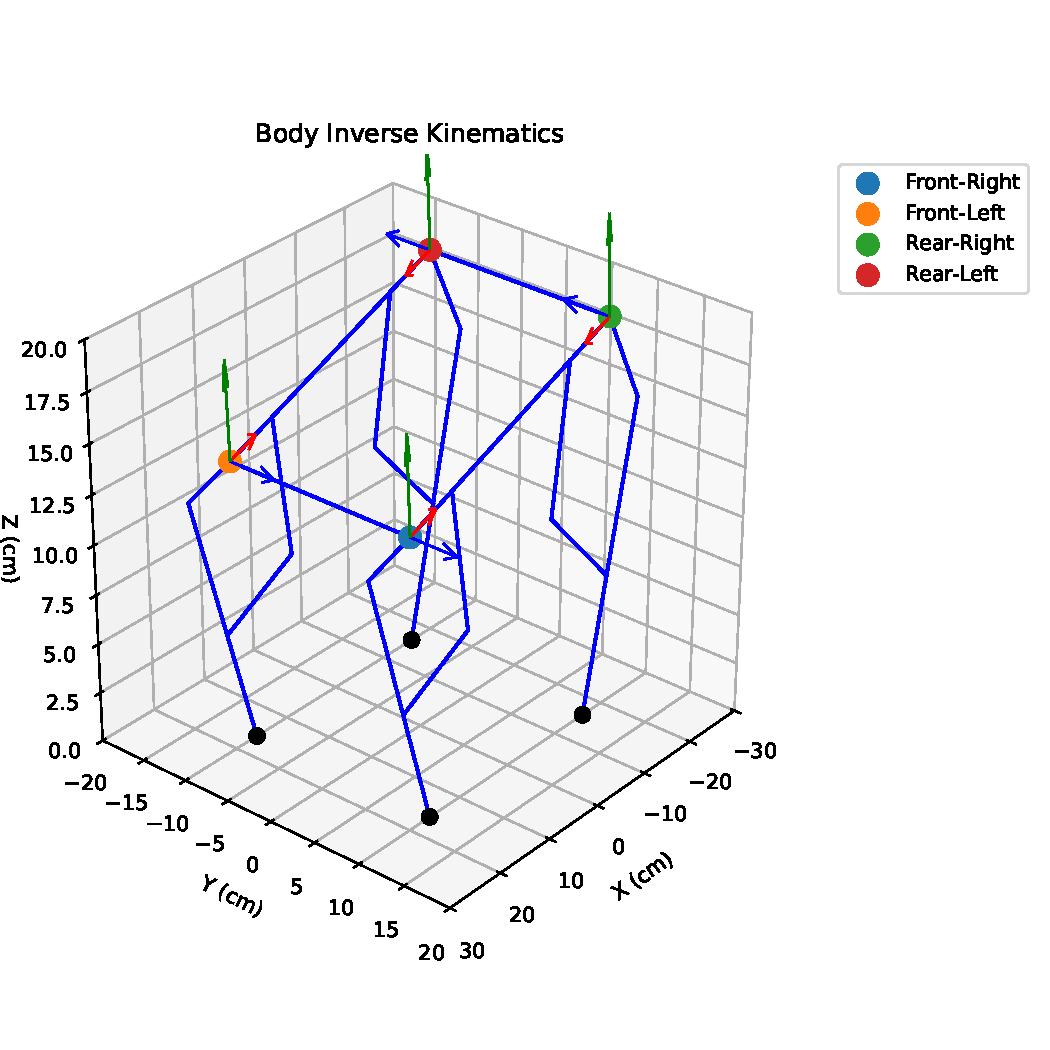
\includegraphics[width=0.55\linewidth]{../../assets/body_inverse_kinematics.pdf}
  \caption{Visualized Body Inverse Kinematics}
  \label{fig:body}
\end{figure}

And for the differential kinematics, we compare the actual end-effector velocities with the desired velocities to ensure the control is accurate.
As shown in the figure below, the vector of actual end-effector velocity fits well with the desired velocity.

\begin{figure}[H]
  \centering
	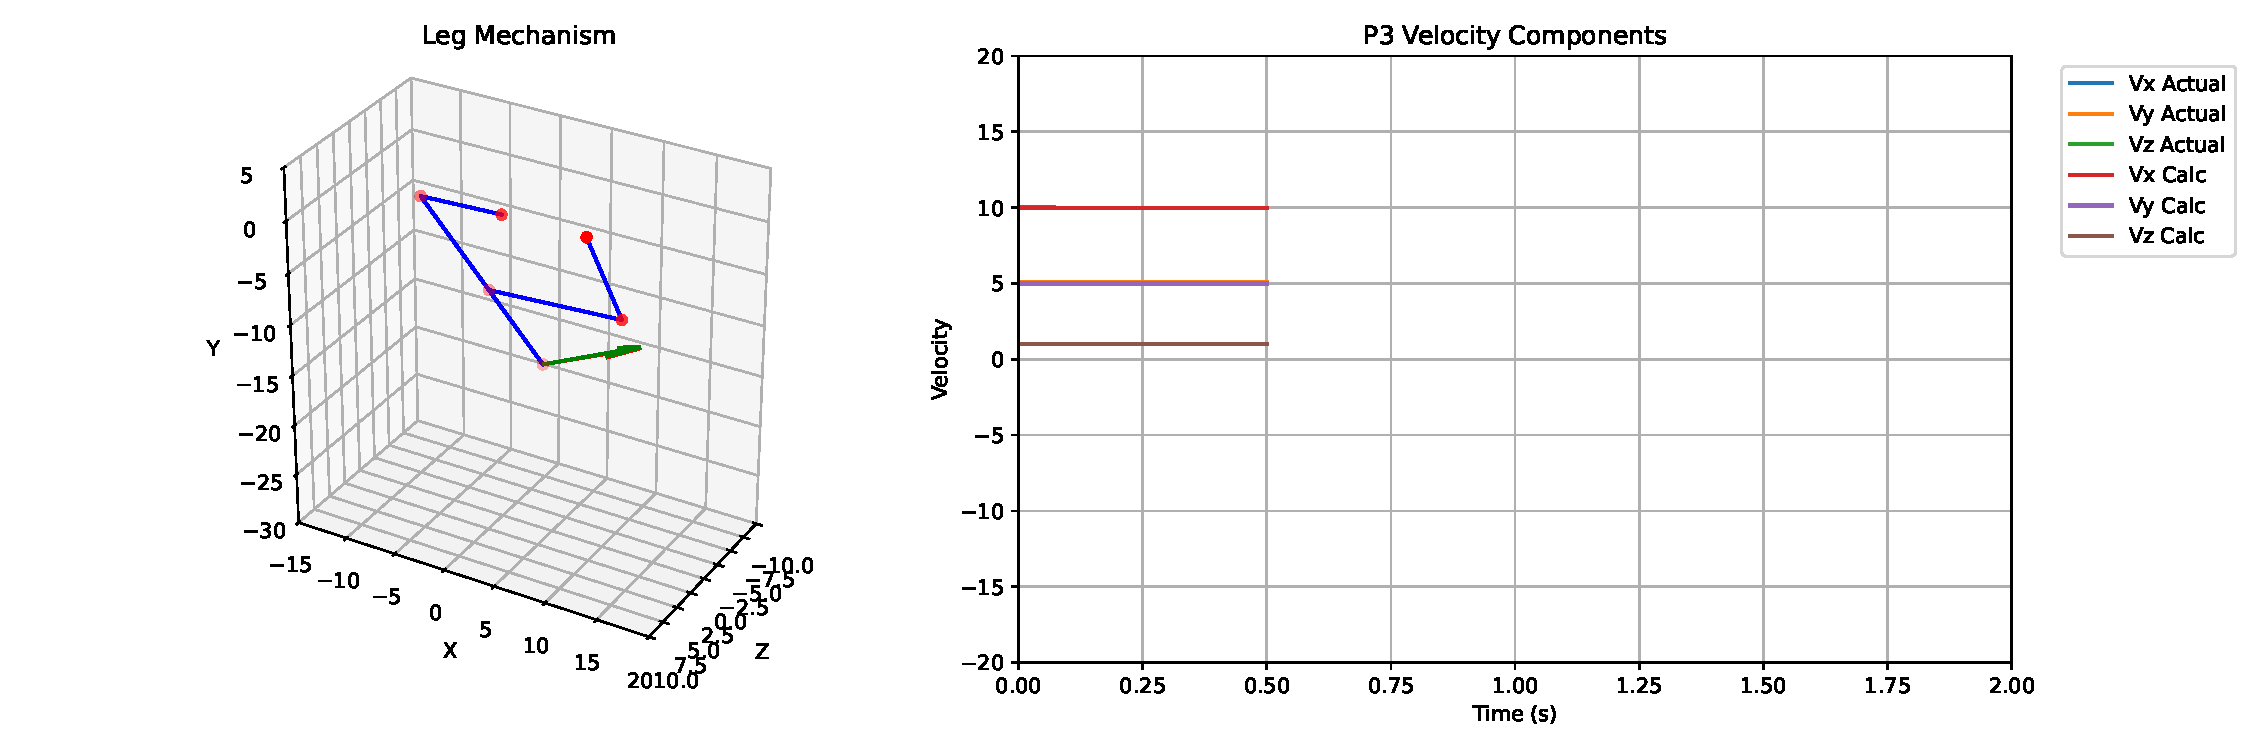
\includegraphics[width=\linewidth]{../../assets/differential_kinematics.pdf}
  \caption{Visualized Differential Kinematics}
  \label{fig:diff}
\end{figure}

Next, we move to the simulation in Pybullet.
Pybullet is a physics engine that allows us to simulate the robot's motion in a realistic environment.
We first use Blender and its extension, Phobos, to transform the solidwork model into a URDF file.
Then we load the URDF file into Pybullet and set up the simulation environment.

\begin{figure}[H]
  \centering
	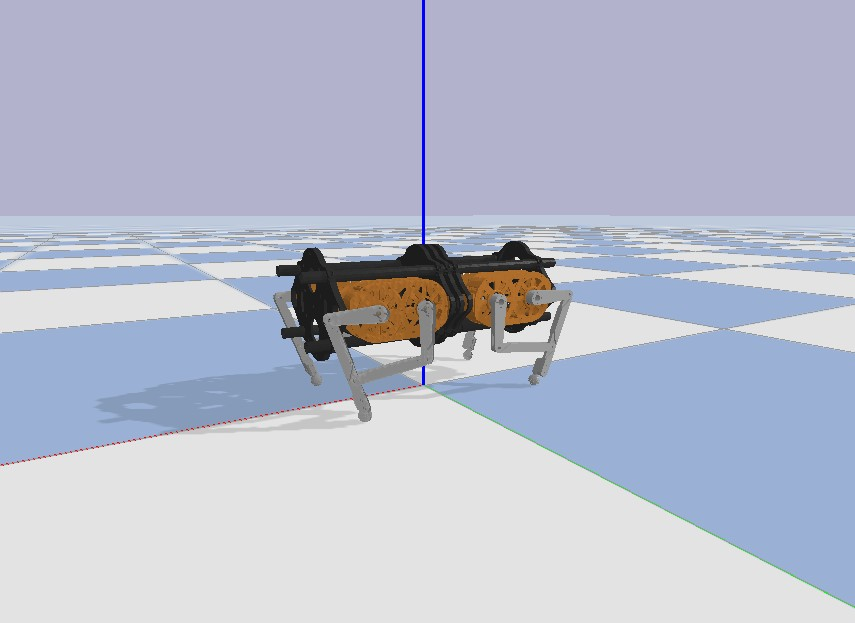
\includegraphics[width=0.6\linewidth]{../../assets/pybullet.jpg}
  \caption{Simulation in Pybullet}
  \label{fig:bullet}
\end{figure}

However, Pybullet does not support the closed chain mechanism of the robot. Therefore, we need to 
cut the each leg into two parts: the upper leg and the lower leg. Then, in the simulation, 
we use the kinematic algorithm to control the position of all links directly to simulate the
closed chain mechanism.

\section{Deep Reinforcement Learning}

To improve Quadson's locomotion stability, we apply deep reinforcement learning with PPO algorithm to generate adaptive offsets for the end-effector positions. This section includes the environment, RL formulation, and training process.

\subsection{Environment Setup}

We developed a custom Gymnasium environment, \texttt{QuadsonEnv}, using Pybullet for simulation. The environment includes:
\begin{itemize}
    \item \textbf{Physics}: Gravity at \(-9.81 \, \text{m/s}^2\), with a plane having friction (lateral: 0.8, spinning: 0.1, rolling: 0.01) and restitution (0.2).
    \item \textbf{Robot}: Quadson with 12 actuated joints, controlled via end-effector offsets.
    \item \textbf{Time Step}: \(1/240 \, \text{s}\) for stable simulation.
\end{itemize}

\subsection{RL Formulation}

The RL problem is defined as follows:

\begin{itemize}
    \item \textbf{Observation Space}: A 29-dimensional vector:
    \begin{itemize}
        \item Body state: roll, pitch, yaw, linear velocity (\(v_x, v_y, v_z\)), angular velocity (\(\omega_x, \omega_y, \omega_z\)) — 9 dimensions.
        \item Joint state: Positions of 12 joints.
        \item Leg phases: Sine and cosine of phases for four legs (LF, RF, LH, RH) — 8 dimensions.
    \end{itemize}
    \item \textbf{Action Space}: A 12-dimensional vector of end-effector offsets (\(x, y, z\) for each leg), bounded between \(-5\) and \(5\) cm.
    \item \textbf{Reward Function}: Combines multiple terms:
    \begin{align*}
			r = & \, 1.0 \cdot \exp(-0.5 (v_x - 0.5)^2) & \text{(forward velocity)} \\
					& - 0.8 \cdot (0.5 v_y^2 + 0.3 \omega_y^2) & \text{(lateral penalty)} \\
					& - 0.8 \cdot (0.5 v_z^2 + 0.3 \omega_z^2) & \text{(vertical penalty)} \\
					& - 1.0 \cdot (40 \text{roll}^2 + 30 \text{pitch}^2 + 5 \text{yaw}^2) & \text{(orientation penalty)} \\
					& - 0.5 \cdot \text{(additional terms for stability and efficiency)}.
    \end{align*}
    Key goals include maintaining forward speed (\(0.5 \, \text{m/s}\)), height (\(0.2 \, \text{m}\)), and reduce the body orientation change during moving.
    \item \textbf{Termination}: Episode ends if roll or pitch exceeds \(45^\circ\), height drops below \(0.1 \, \text{m}\), or 4500 steps are reached.
\end{itemize}

\subsection{System Design}

\begin{figure}[H]
  \centering
	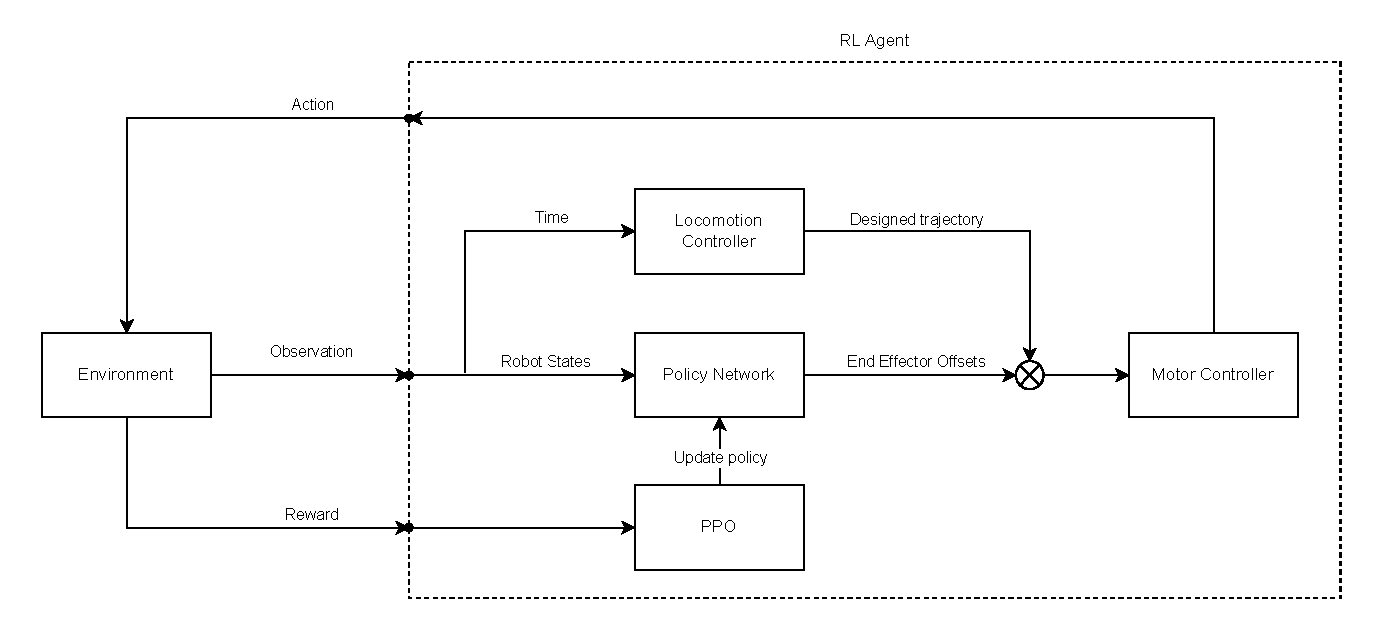
\includegraphics[width=0.9\linewidth]{../../assets/system_diagram.pdf}
  \caption{System Block Diagram}
  \label{fig:system}
\end{figure}

\subsection{Training Process}

We use the Proximal Policy Optimization (PPO) algorithm from Stable Baselines3 due to its stability and sample efficiency.
Hyperparameters (e.g., learning rate, batch size) are under optimization during training.

\begin{figure}[H]
  \centering
	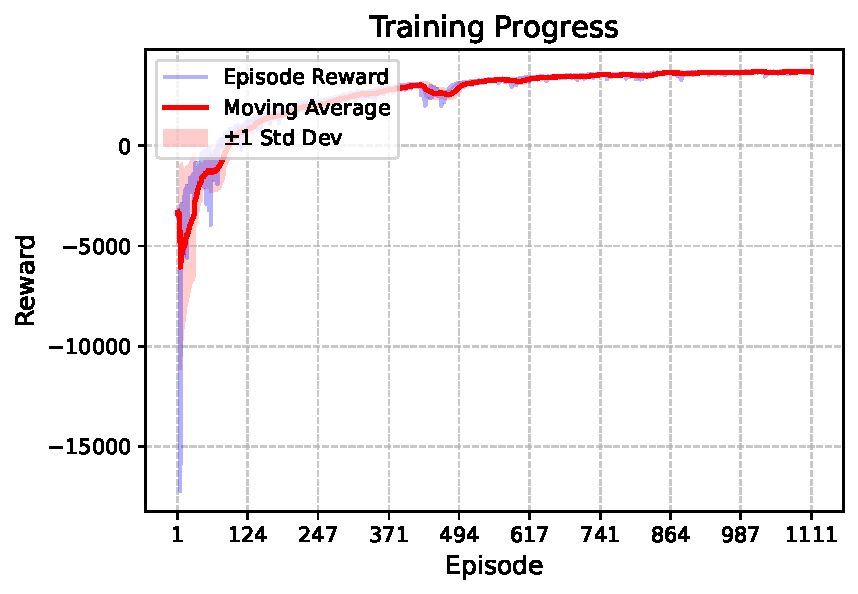
\includegraphics[width=0.5\linewidth]{../../assets/rl_training_progress.pdf}
  \caption{Reward}
  \label{fig:reward}
\end{figure}

\subsection{Results}

In the training, the agent performs 5000000 steps in total to interact with enviroment and update the network. 
Figure \ref{fig:compare_vel} shows that the forward velocity (vx) has increased, but it still not achieve the target velocity of 0.5m/s.
This could be due to limitations in the locomotion settings, where the model can only adjust the position of the end effector. To achieve the desired velocity, 
further tuning to the gait's length and timing is needed.

For vertical velocity (vz), both standard deviation and average have decreased slightly. Although the improvement is not significant but it still represents progress.
To further improve the stability, we may need to fine-tune the reward function or increase the depth of the deep network.

\begin{figure}[H]
	\centering
	\begin{subfigure}[b]{0.7\textwidth}
			\centering
			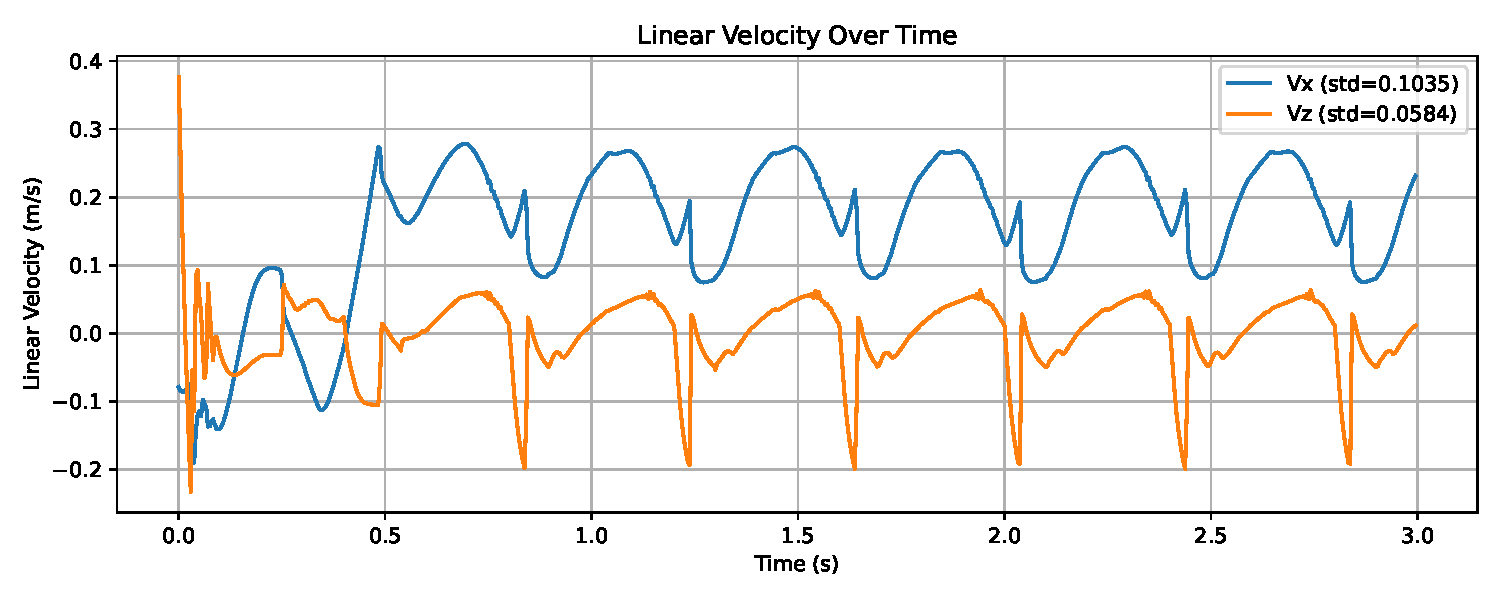
\includegraphics[width=\linewidth]{../../assets/alg_vel.pdf}
			\caption{Locomotion Algorithm}
	\end{subfigure}
	\vfill
	\begin{subfigure}[b]{0.7\textwidth}
			\centering
			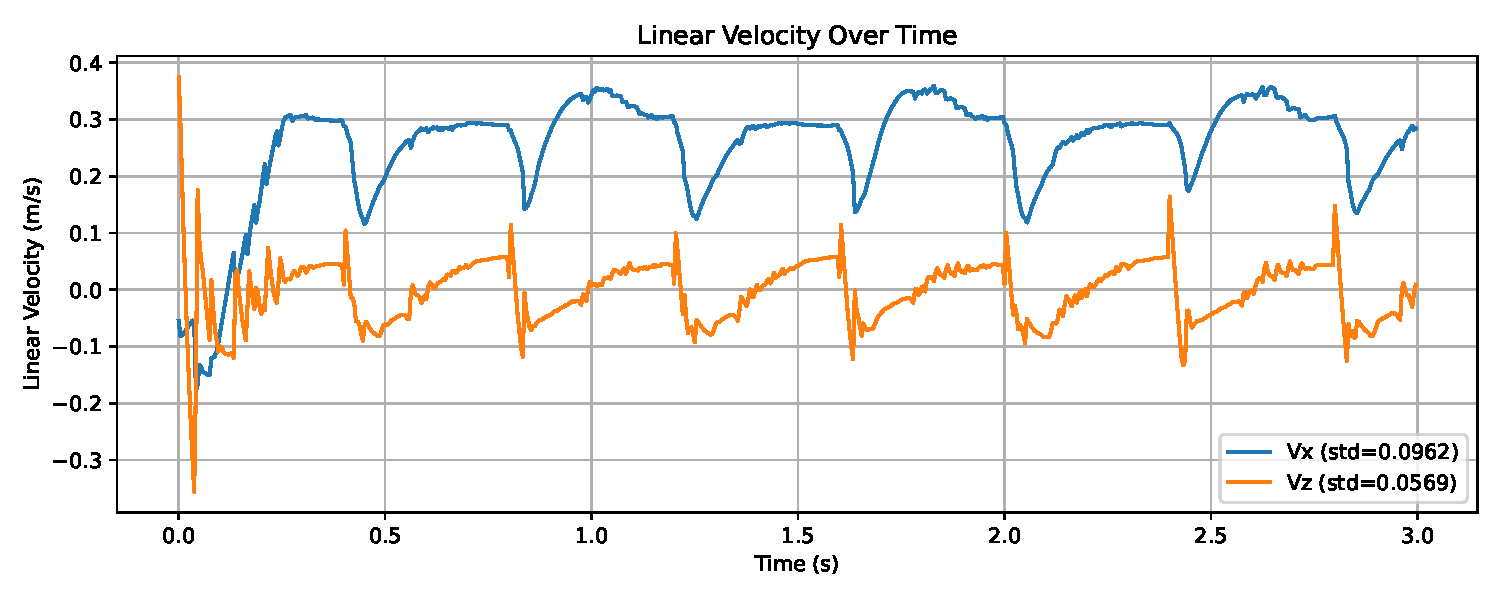
\includegraphics[width=\linewidth]{../../assets/model_vel.pdf}
			\caption{DRL Model}
	\end{subfigure}
	\caption{Velocity Comparison of Different Control Methods Over a 3-Second Trial.}
	\label{fig:compare_vel}
\end{figure}

Regarding the orientation stability, there's a significant improvement. As shown in Figure \ref{fig:compare_ori},
both the roll and pitch averages are now close to zero, with their standard deviations reduced by over 80\%.

\begin{figure}[H]
	\centering
	\begin{subfigure}[b]{\textwidth}
		\centering
		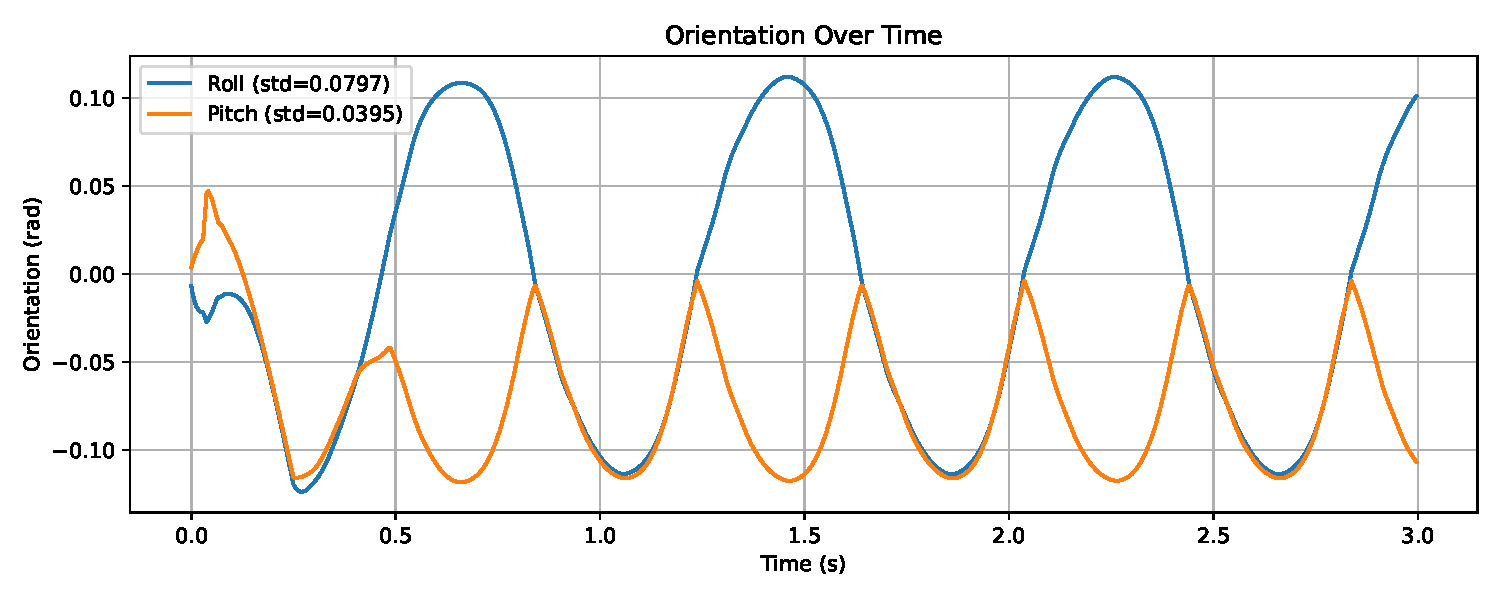
\includegraphics[width=0.7\linewidth]{../../assets/alg_ori.pdf}
		\caption{Locomotion Alogrithm}
	\end{subfigure}
	\vfill
	\begin{subfigure}[b]{\textwidth}
		\centering
		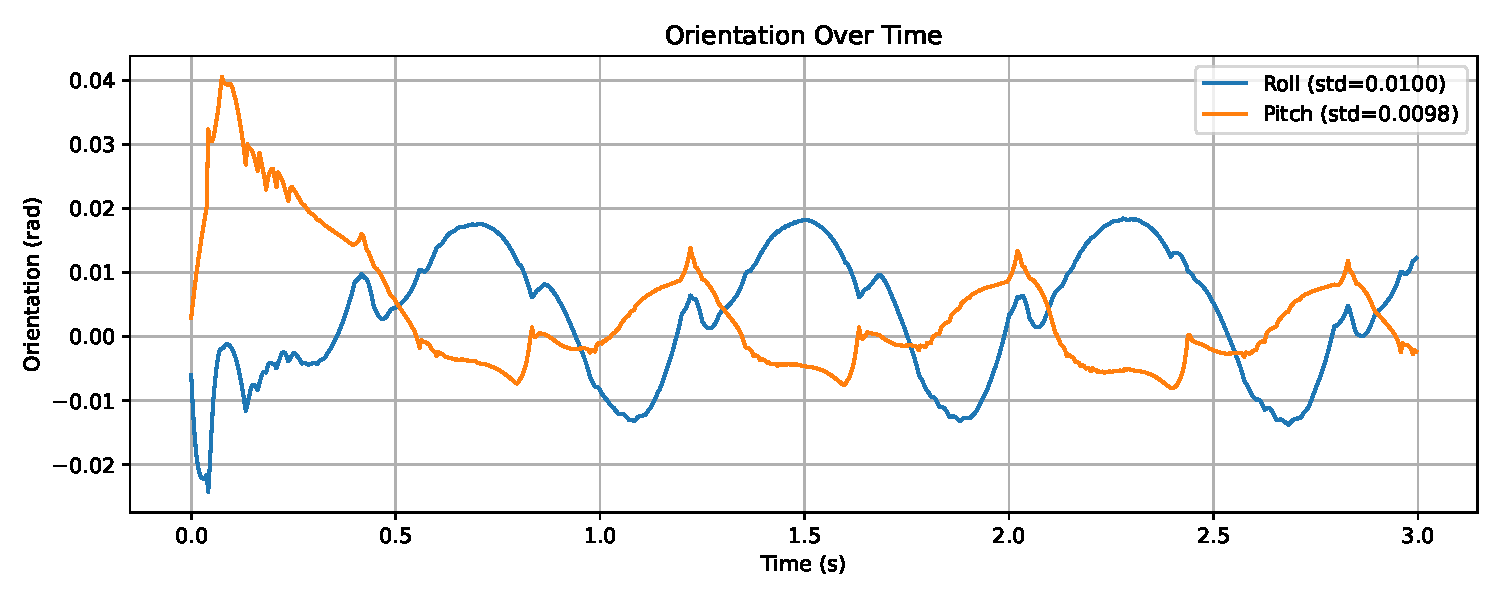
\includegraphics[width=0.7\linewidth]{../../assets/model_ori.pdf}
		\caption{RL Model}
	\end{subfigure}
	\caption{Orientation Comparision of Different Control Method Over a 3-Second Trial.}
	\label{fig:compare_ori}
\end{figure}

\section{Future Work}

So far, we have implemented and valided kinematic algorithms, 
setting up a virtual environment for motion testing and reinforcement 
learning training. The Deep RL model aims to improve locomotion stability with 
adaptive gait offsets. The next steps are:

\begin{enumerate}
	\item \textbf{Simulation-to-Reality Transfer}: Deploy algorithms and model to the physical robot, deal with factors like friction and motor latency through tuning or domain randomization.
	\item \textbf{Walking Stability}: Refine RL policy to handle the movement in different terrians, such as slopes or uneven surfaces.
	\item \textbf{Sensor Integration}: Add IMU or LiDAR for real-time feedback and obstacle detection.
	\item \textbf{Expanded Locomotion}: Enable movement in various directions other than forward, such as sideways.
	\item \textbf{Recovery Mechanisms}: Enable self-righting or failure adaptation to protect the robot from falling.
	\item \textbf{Migrate to Isaac Gym}: Transition the simulation environment to Isaac Gym for better scalability and performance, using its advanced physics engine and GPU acceleration for more efficient training and testing.
\end{enumerate}

These steps will transition Quadson from simulation to a functional real-world robot.

\section{Conclusion}

We developed a kinematic framework for Quadson, covering forward, inverse, differential, and body kinematics, alongside locomotion control. These algorithms were validated in Pybullet, where simulations confirmed accurate end-effector positioning and velocity tracking. 
To enhance stability, we initiated deep reinforcement learning with PPO to adjust gait offsets, with training ongoing. Despite Pybullet's limitation with closed-chain mechanisms, we adapted by controlling link positions directly. This work establishes Quadson as a platform for robotic motion studies, 
blending classical kinematics with Deep RL. The next step is real-world deployment, building on this foundation to achieve practical functionality.

\end{document}